\documentclass[12pt,a4paper]{article}
\usepackage[T1]{fontenc}
\usepackage[utf8]{inputenc}
\usepackage[polish]{babel}
\usepackage{lmodern}
\usepackage{geometry}
\usepackage{graphicx}
\usepackage{float}
\usepackage{booktabs}
\usepackage{array}
\usepackage{hyperref}
\usepackage{xcolor}
\geometry{margin=2.5cm}
\hypersetup{
    colorlinks=true,
    linkcolor=black,
    urlcolor=blue,
    pdftitle={Projekt 2 - Rozpoznawanie cz{\l}owieka na podstawie obrazu t\k{e}cz\'owki},
    pdfauthor={Aleksander Brandt, Kamila Wieckowksa}
}

\title{\vspace{-1.8cm}\Huge Projekt 2\\[0.3cm]\LARGE Rozpoznawanie cz{\l}owieka na podstawie obrazu t\k{e}cz\'owki}
\author{Aleksander Brandt \and Kamila Wieckowksa}
\date{30 kwietnia 2026}

\begin{document}

\begin{titlepage}
    \centering
    {\Large Biometria\par}
    \vspace{1.8cm}
    {\Huge\bfseries Projekt 2\par}
    \vspace{0.4cm}
    {\LARGE Rozpoznawanie cz{\l}owieka na podstawie obrazu t\k{e}cz\'owki\par}
    \vspace{2cm}
    {\large
    \begin{tabular}{rl}
    Autorzy: & Aleksander Brandt \\
             & Kamila Wieckowksa \\
    Data:    & 30 kwietnia 2026 \\
    \end{tabular}\par}
    \vfill
    {\large Segmentacja, kodowanie i por\'ownywanie wzorc\'ow t\k{e}cz\'owki na zbiorze MMU Iris Dataset\par}
\end{titlepage}

\section{Cel pracy}
Celem pracy by{\l}o zbudowanie kompletnego pipeline'u rozpoznawania t\k{e}cz\'owki: od przygotowania obrazu oka i segmentacji jego najwa\.zniejszych granic, przez normalizacj\k{e} oraz zakodowanie tekstury, a\.z do por\'ownania otrzymanych kod\'ow i oceny skuteczno\'sci metody na zbiorze MMU Iris Dataset.

\section{Opis metody}
Zastosowany pipeline sk{\l}ada si\k{e} z kilku kolejnych etap\'ow. Najpierw obraz jest zamieniany do skali szaro\'sci, lekko wyg{\l}adzany i binaryzowany osobno dla potrzeby segmentacji \'zrenicy i t\k{e}cz\'owki. Nast\k{e}pnie wyznaczana jest granica \'zrenicy na podstawie analizy ciemnych obszar\'ow obrazu, a granica zewn\k{e}trzna t\k{e}cz\'owki jest okre\'slana na podstawie radialnego profilu jasno\'sci.

Po segmentacji pier\'scie\'n t\k{e}cz\'owki jest rozwijany do postaci prostok\k{a}tnej. W analizie pomijane s\k{a} g\'orne i dolne fragmenty bardziej podatne na zas{\l}oni\k{e}cie przez powieki i rz\k{e}sy. Otrzymany obraz normalizowany ma rozmiar $128 \times 128$ i jest dzielony na 8 pas\'ow radialnych.

Z ka\.zdego pasa budowany jest sygna{\l} 1D opisuj\k{a}cy zmiany jasno\'sci po k\k{a}cie. Do kodowania wykorzystano filtr Gabora 1D. Znak cz\k{e}\'sci rzeczywistej i urojonej odpowiedzi filtra tworzy binarny kod t\k{e}cz\'owki, natomiast modu{\l} odpowiedzi s{\l}u\.zy do budowy maski wiarygodno\'sci bit\'ow. Por\'ownanie dw\'och pr\'obek odbywa si\k{e} za pomoc\k{a} maskowanej odleg{\l}o\'sci Hamminga z kompensacj\k{a} niewielkiego przesuni\k{e}cia k\k{a}towego.

\section{Konfiguracja eksperymentu}
W finalnej konfiguracji wykorzystano nast\k{e}puj\k{a}ce parametry:
\begin{itemize}
    \item \texttt{iris\_threshold\_divisor\_xi = 5.0},
    \item \texttt{pupil\_threshold\_divisor\_xp = 7.0},
    \item \texttt{radial\_bands = 8},
    \item \texttt{angular\_samples = 128},
    \item \texttt{radial\_samples\_per\_band = 16},
    \item \texttt{gabor\_frequency = 0.0245436926},
    \item \texttt{max\_angular\_shift = 8},
    \item \texttt{verify\_threshold = 0.216}.
\end{itemize}

Warto\'s\'c cz\k{e}stotliwo\'sci filtra Gabora odpowiada przyj\k{e}tej rozdzielczo\'sci k\k{a}towej i w praktyce da{\l}a stabilne, rozr\'o\.znialne odpowiedzi na badanym zbiorze.

\section{Zbi\'or danych}
Ko\'ncow\k{a} walidacj\k{e} wykonano na pe{\l}nym zbiorze \textbf{MMU Iris Dataset}, zapisanym lokalnie w strukturze katalog\'ow:
\begin{verbatim}
MMU-Iris-Database/<osoba>/<left|right>/<plik>.bmp
\end{verbatim}

W badaniu wykorzystano:
\begin{itemize}
    \item 45 os\'ob,
    \item 2 oczy na osob\k{e},
    \item 5 obraz\'ow dla ka\.zdego oka,
    \item {\l}\k{a}cznie 450 obraz\'ow i 90 klas t\k{e}cz\'owki.
\end{itemize}

\begin{figure}[H]
    \centering
    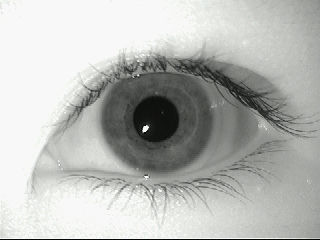
\includegraphics[width=0.42\textwidth]{zdjecia/mmu_wejscie/aeval1.png}\hfill
    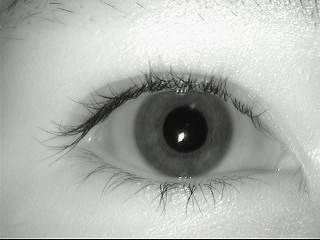
\includegraphics[width=0.42\textwidth]{zdjecia/mmu_wejscie/aevar1.png}
    \caption{Przyk{\l}adowe obrazy wej\'sciowe z MMU Iris Dataset.}
\end{figure}

\section{Implementacja}
Implementacja zosta{\l}a przygotowana jako niewielki pakiet Python. G{\l}\'owny punkt wej\'scia znajduje si\k{e} w pliku \texttt{src/iris/main.py}, natomiast zasadnicza logika etap\'ow segmentacji, normalizacji, kodowania i por\'ownywania zosta{\l}a zebrana w pliku \texttt{src/iris/pipeline.py}. Konfiguracja jest wczytywana z plik\'ow JSON, a poprawno\'s\'c wybranych funkcji pomocniczych i element\'ow pipeline'u jest sprawdzana przez testy jednostkowe.

Walidacja by{\l}a wykonywana komendami:
\begin{verbatim}
python src\iris\main.py --config config\mmu_dataset_template.json run
python -m unittest discover -s tests -p "test_*.py"
\end{verbatim}

Zestaw test\'ow obejmuje 9 przypadk\'ow i przechodzi w ca{\l}o\'sci bez b{\l}\k{e}d\'ow.

\section{Wyniki jako\'sciowe}
Segmentacja dzia{\l}a stabilnie na pe{\l}nym zbiorze MMU i prowadzi do poprawnego rozwini\k{e}cia t\k{e}cz\'owki do postaci prostok\k{a}tnej. W przeprowadzonej walidacji end-to-end wszystkie 450 obraz\'ow przesz{\l}o przez etapy segmentacji, normalizacji i kodowania.

\begin{figure}[H]
    \centering
    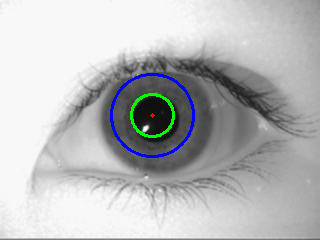
\includegraphics[width=0.46\textwidth]{zdjecia/mmu_wyniki/aeval1_iris_circle_overlay.png}\hfill
    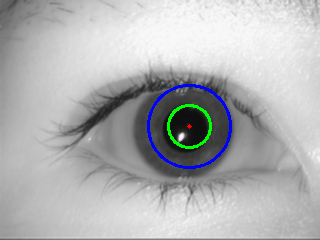
\includegraphics[width=0.46\textwidth]{zdjecia/mmu_wyniki/aevar1_iris_circle_overlay.png}
    \caption{Przyk{\l}adowe wyniki segmentacji granicy \'zrenicy i t\k{e}cz\'owki dla danych MMU.}
\end{figure}

\begin{figure}[H]
    \centering
    
\includegraphics[width=0.24\textwidth]{zdjecia/mmu_wyniki/1_left_aeval1_normalized.png}
    \caption{Przyk{\l}ad znormalizowanej i rozwini\k{e}tej t\k{e}cz\'owki.}
\end{figure}

\section{Wyniki ilo\'sciowe}
Najwa\.zniejsze wyniki uzyskane dla ko\'ncowej konfiguracji przedstawiono w tabeli.

\begin{center}
\begin{tabular}{>{\raggedright\arraybackslash}p{0.56\textwidth}p{0.22\textwidth}}
\toprule
Miara & Warto\'s\'c \\
\midrule
Liczba par genuine & 900 \\
Liczba par impostor & 100125 \\
\'Srednia odleg{\l}o\'s\'c genuine & 0.1781 \\
\'Srednia odleg{\l}o\'s\'c impostor & 0.2272 \\
Odchylenie standardowe genuine & 0.0410 \\
Odchylenie standardowe impostor & 0.0144 \\
EER & 0.2066 \\
Pr\'og EER & 0.2160 \\
Accuracy identyfikacji leave-one-out & 0.8578 \\
\bottomrule
\end{tabular}
\end{center}

\begin{figure}[H]
    \centering
    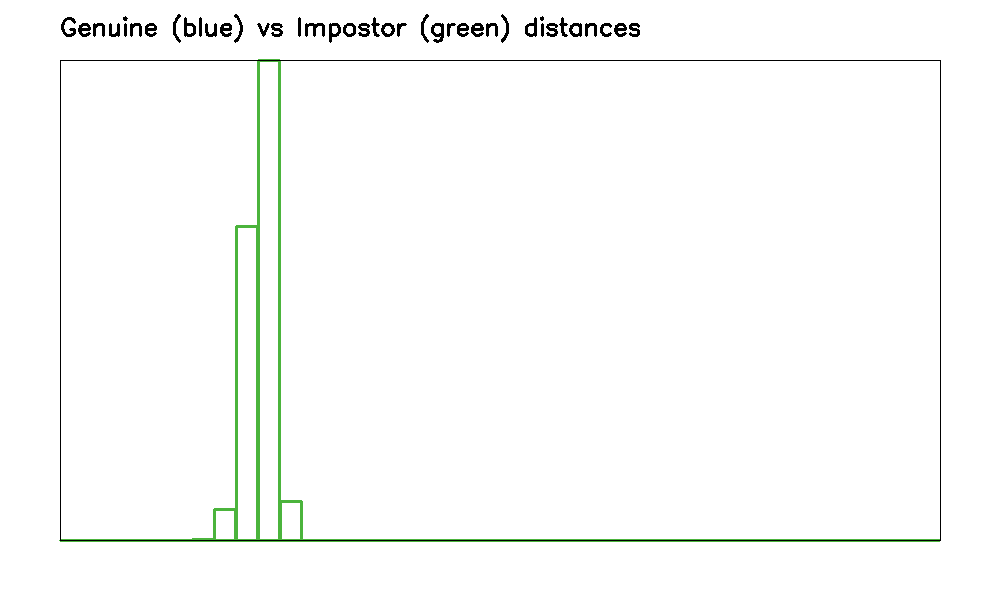
\includegraphics[width=0.82\textwidth]{zdjecia/mmu_wyniki/distance_histogram_mmu.png}
    \caption{Histogram odleg{\l}o\'sci Hamminga dla par genuine i impostor na MMU.}
\end{figure}

\begin{figure}[H]
    \centering
    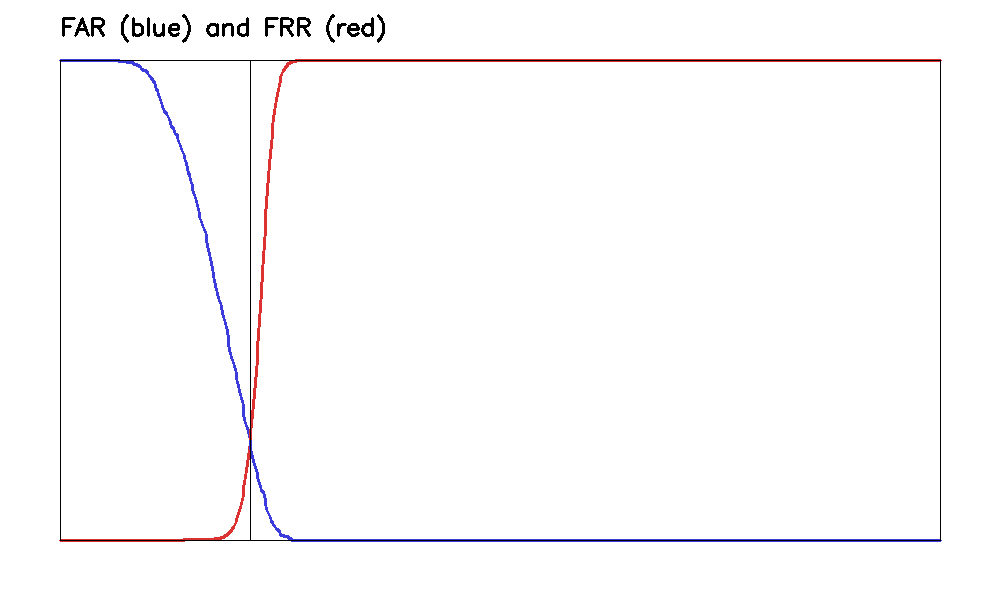
\includegraphics[width=0.82\textwidth]{zdjecia/mmu_wyniki/far_frr_curve_mmu.png}
    \caption{Krzywe FAR i FRR oraz punkt EER dla finalnej konfiguracji.}
\end{figure}

\section{Dyskusja wynik\'ow}
\'Srednia odleg{\l}o\'s\'c dla par genuine jest wyra\'znie mniejsza ni\.z dla par impostor, co potwierdza, \.ze kod t\k{e}cz\'owki przenosi informacj\k{e} rozr\'o\.zniaj\k{a}c\k{a} poszczeg\'olne klasy. Jednocze\'snie histogram pokazuje cz\k{e}\'sciowe nak{\l}adanie si\k{e} rozk{\l}ad\'ow, co jest zgodne z uzyskanym poziomem EER. W praktyce oznacza to, \.ze system rozpoznaje wzorce poprawnie w wi\k{e}kszo\'sci przypadk\'ow, ale przy trudniejszych pr\'obkach nadal pojawiaj\k{a} si\k{e} pomy{\l}ki wynikaj\k{a}ce g{\l}\'ownie z niedoskona{\l}o\'sci segmentacji i z naturalnej zmienno\'sci obraz\'ow oka.

Wynik identyfikacji leave-one-out na poziomie 0.8578 wskazuje, \.ze metoda dobrze radzi sobie w scenariuszu wyszukiwania najlepszego dopasowania w galerii, chocia\.z pozostaje miejsce na popraw\k{e} jako\'sci przez dok{\l}adniejsze maskowanie obszar\'ow zak{\l}\'oconych lub dalsze strojenie kodowania.

\section{Wnioski}
Opracowany system realizuje pe{\l}ny proces rozpoznawania t\k{e}cz\'owki: od obrazu wej\'sciowego do decyzji o podobie\'nstwie lub identyfikacji. Najbardziej czu{\l}ymi elementami pipeline'u okaza{\l}y si\k{e} segmentacja oraz dob\'or parametr\'ow kodowania, poniewa\.z to one w najwi\k{e}kszym stopniu wp{\l}ywaj\k{a} na jako\'s\'c otrzymanego szablonu.

Ko\'ncowa walidacja na pe{\l}nym MMU Iris Dataset potwierdzi{\l}a, \.ze implementacja dzia{\l}a stabilnie i pozwala uzyska\'c sp\'ojne wyniki zar\'owno w trybie verification, jak i identification. Otrzymane rezultaty pokazuj\k{a}, \.ze przyj\k{e}ta metoda jest poprawna i daje sensown\k{a} jako\'s\'c rozpoznawania dla danych wykorzystanych w eksperymencie.

\end{document}
